\chapter{Experiments}
We compare the trajectories of the bodies in the baseline control systems to those generated by control systems that represent preliminary hypotheses. By examining the similarities and differences between the trajectories, we can verify whether the preiliminary hypotheses are sufficient for producing the head-bobbing behaviors seen in pigeons.

\section{Dimensions of the Pigeon Model}
  Our pigeon model's dimensions and orientations are set at static values for all experiments, as shown in Figure \ref{fig:pigeon_dimension}.
    \begin{figure}[H]
        \centering
        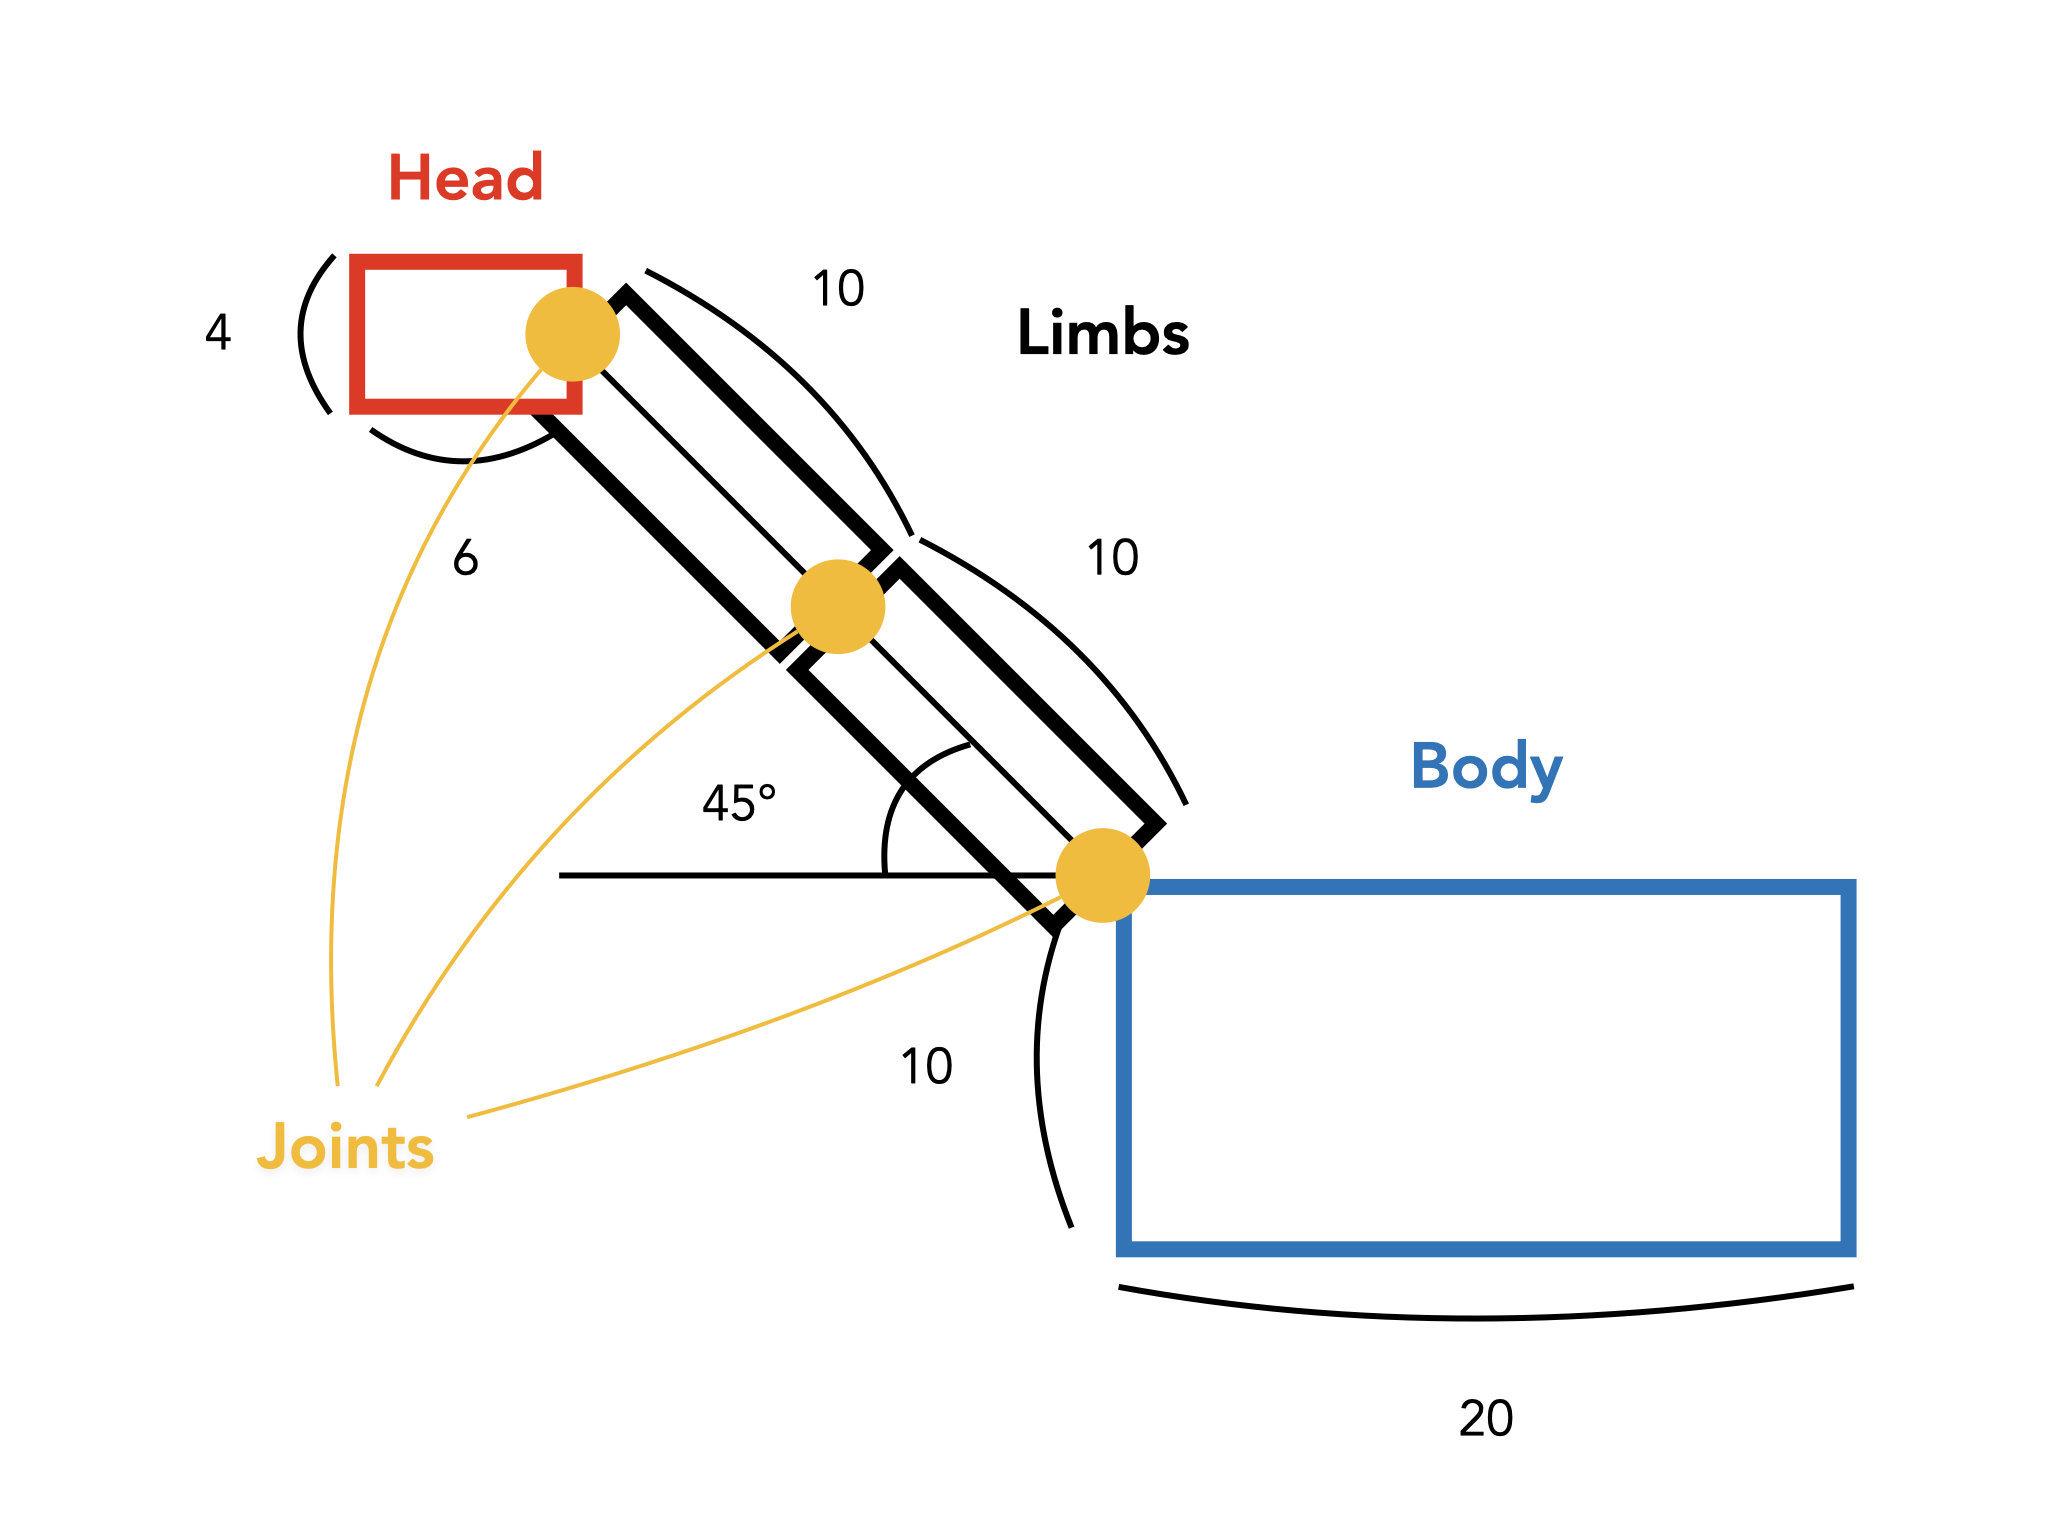
\includegraphics[width=1\textwidth]{figures/pigeon_diagram/pigeon_diagram_001.png}
        \caption{Diagram of the pigeon model}
        \label{fig:pigeon_dimension}
    \end{figure}
  Additionally, the pigeon's head relative to the body is facing the negative direction relative to the x-axis.
  The widths and heights of each limb, head, and body are $(10, 4)$, $(6, 4)$, $(20, 10)$ respectively.
  The initial angles of each limb are oriented at 45 degrees relative to the x-axis, and both the head and the body are oriented parallel to the x axis.
  The body's initial position is at the origin, and is set to move at a constant speed in the negative direction along the x-axis.

\section{Experiment Environments}
% details on all 5 params and reward function differences
  We trained a total of 5 reinforcement learning agents to control the pigeon model: 1 agent for the case where the model is given the baseline task given an unmoving body, 2 agents for cases where the model is given the same task with the body speed of 1, 2 agents for cases where the model is tasked to move its joints to maximize the reward function $r_{fifty\_fifty}$, as defined in the previous chapter, under the body speed of 0 and 1 respectively.

  % head target trajectory tracking
    Several additional variables are defined for the pigeon to execute the baseline task as shown in \ref{fig:pigeon_target}.
      \begin{figure}[H]
          \centering
          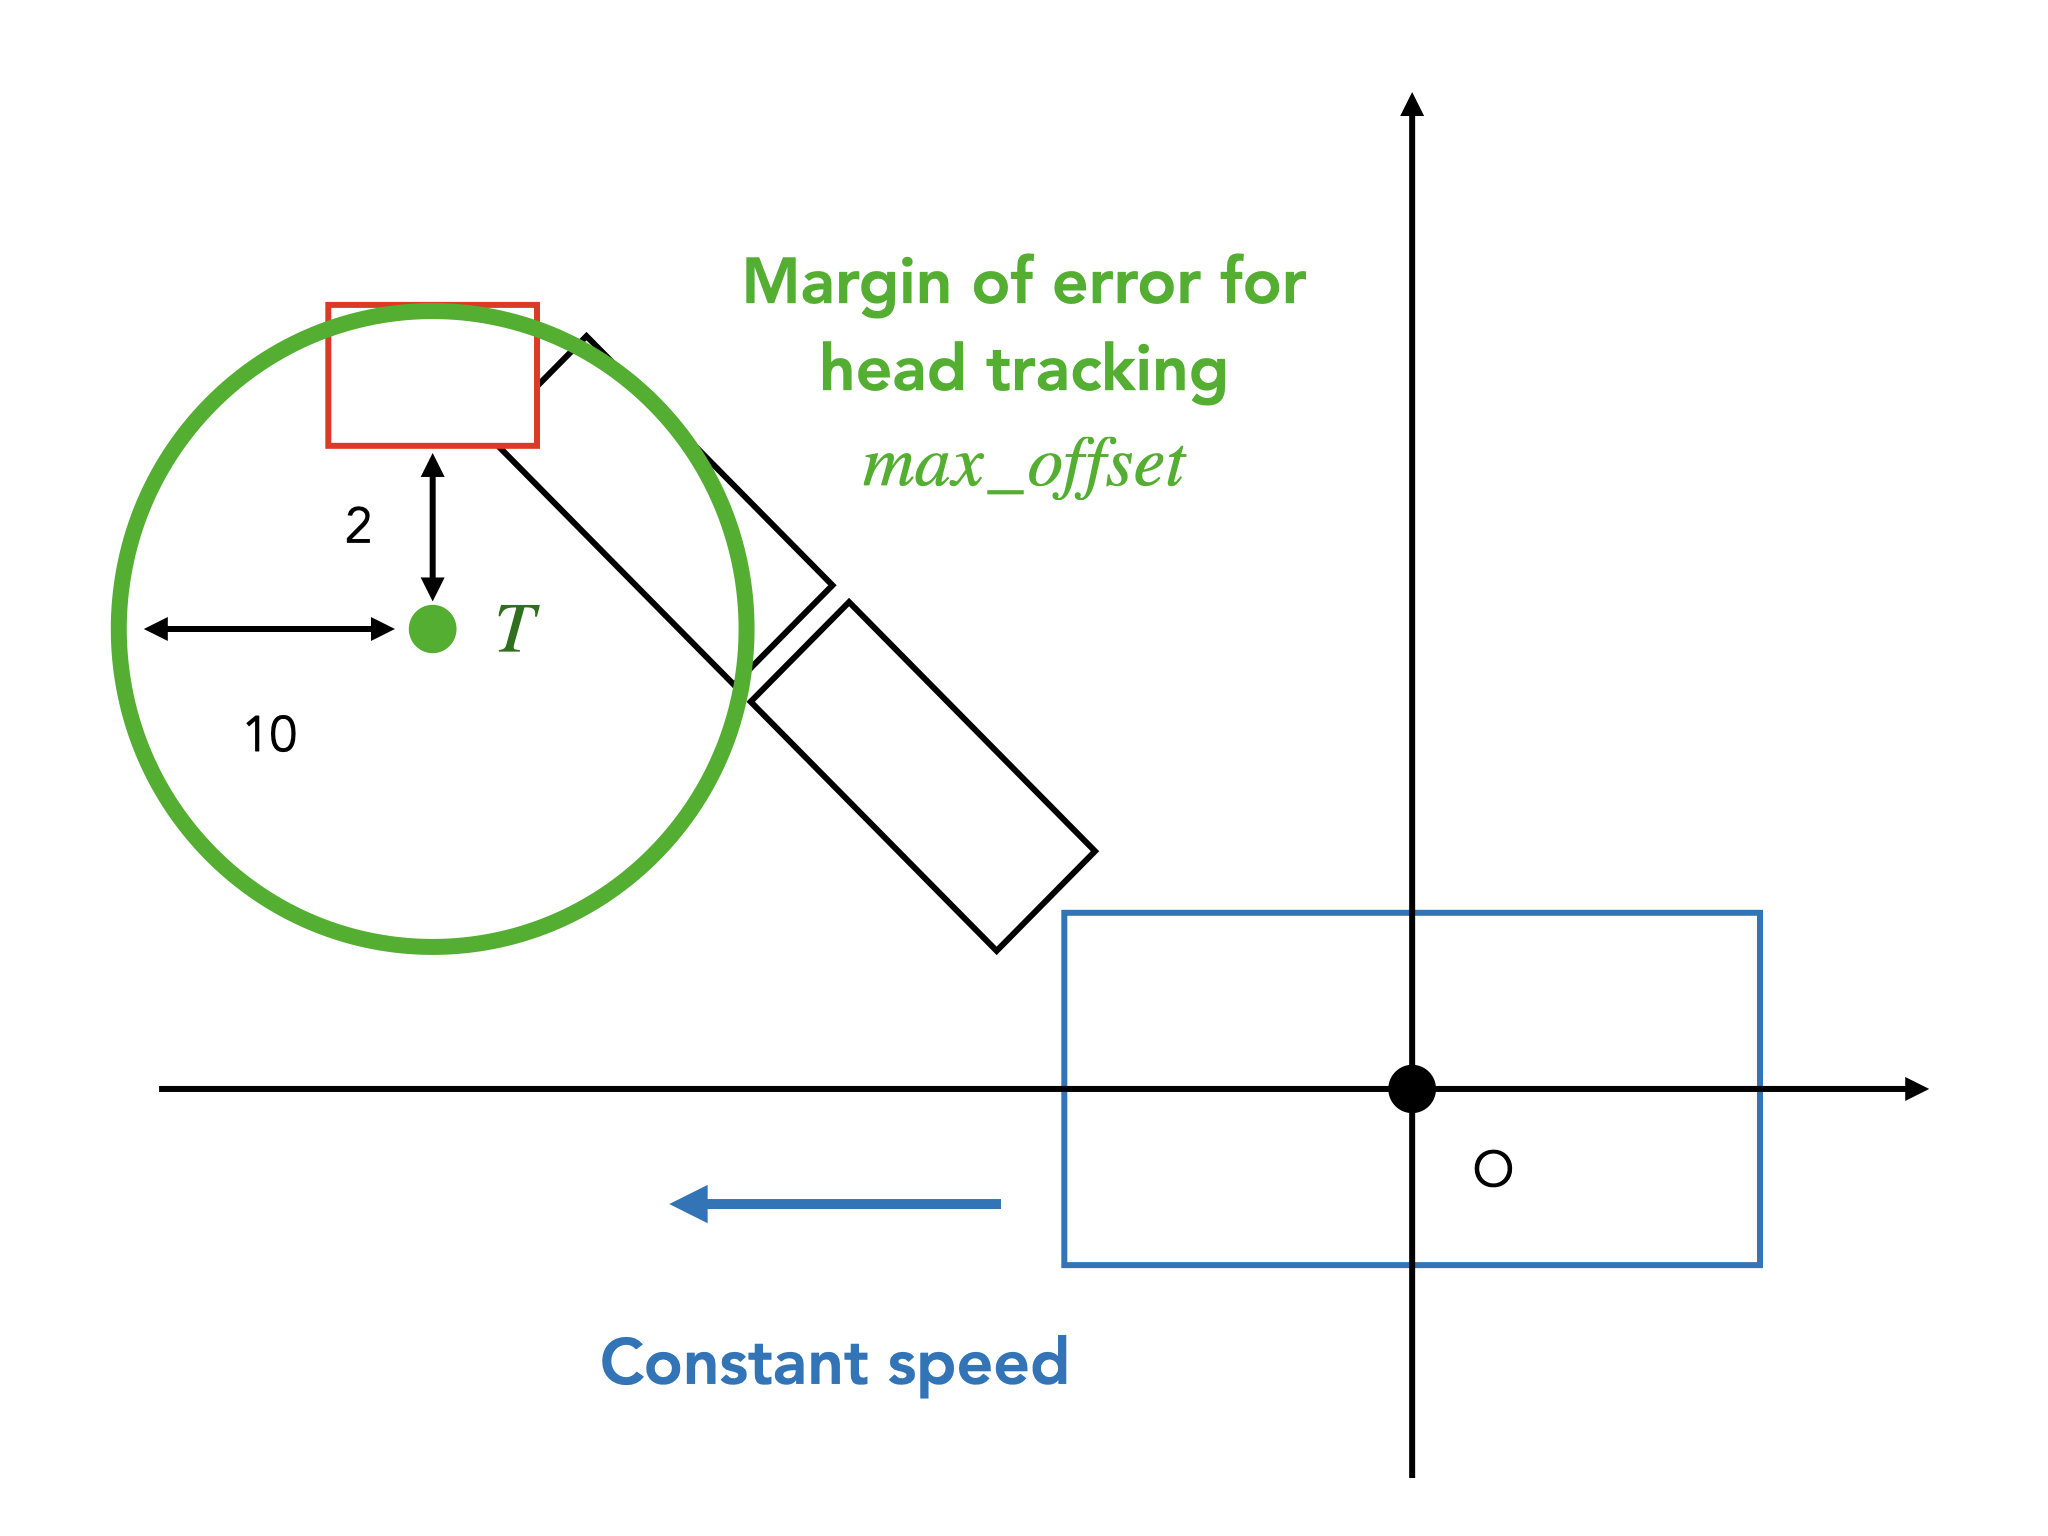
\includegraphics[width=1\textwidth]{figures/pigeon_diagram/pigeon_diagram_002.png}
          \label{fig:pigeon_target}
          \caption{Head trajectory tracking}
      \end{figure}
    $T$ is set at $(0, -2)$ relative to the initial position of the head.
    We set the threshold value for the distance between the target position and the torso's position to 10. As mentioned in the previous chapter, when the the said distance is below the threshold value, $T$ is reset to be the same position relative to the body as its initial position.
    We set a value $max\_offset$ that represents the margin of error between $T$ and the position of the head.

    % speed = 0
      % _head_stable_manual_reposition_strict_angle
        For the case with an unmoving body, we define a function that generates positive rewards only for timesteps where the distance between the head and $T$ is within $max\_offset = 0.5$. Each reward is bounded within $[0, 1]$ and scaled based on the level of alignment to the x-axis.
          \begin{equation}
              {r_{head\_stable\_manual\_reposition\_strict\_angle}}_t =
              \begin{cases}
                  1 - \frac {\alpha_t} \pi & \text{if $\alpha_t < \frac \pi 6$} \\
                  0 & \text{otherwise}
              \end{cases}
          \end{equation}
        where $\alpha_t$ is the angle of the head at timestep $t$.

    % speed = 1
      % _head_stable_manual_reposition
        For the speed of 1, unlike the case with the unmoving body, $max\_offset = 1$.
        Additionally, alongside $r_{head\_stable\_manual\_reposition\_strict\_angle}$, we define a looser reward function that generates positive rewards as long as the head is within the set margin of error around the target location.
        It is expected that this function would serve as an alternate less strict to the former reward function that produce similar behaviors.
        \begin{equation}
          \begin{aligned}
            {r_{head\_stable\_manual\_reposition}}_t = {r_{head\_stable\_manual\_reposition\_strict\_angle}}_t + \\
              \begin{cases}
                  1 - \frac {\delta_t} {max\_offset} & \text{$\delta_t < max\_offset$} \\
                  0 & \text{otherwise}
              \end{cases}
          \end{aligned}
        \end{equation}
        where $\delta_t$ is the distance between the head and $T$ at timestep $t$.

  % _fifty_fifty
    Preliminary hypotheses regarding retinal stabilization and motion parallax are depicted as the reward function $r_{fifty\_fifty}$. The reward function is used to train agents that represent behaviors derived from such hypotheses under the conditions of both speeds 0 and 1. For both cases, $max\_offset = 1$.
    % external objects
      3 points and their positions are defined to represent 1 static and 2 dynamic objects placed on the surrounding environment of the pigeon.
      The static object's position is $(-30.0, 30.0)$, and the 2 dynamic objects' positions are $(-30.0, 60.0)$, $(-60.0, 30.0)$. The former dynamic object moves at speed 1 in the positive direction along the x-axis, while the latter moves at the same speed in the negative direction along the x-axis.

We constructed OpenAI Gym environments \lstinline|PigeonEnv3Joints| and \lstinline|PigeonRetinalEnv| for conducting reinforcement learning based on the baseline and preliminary hypotheses, respectively.
  Details regarding the environments' code are in the Appendix.

\section{Reinforcement Learning}
We used SAC to conduct batch training on each deep neural network agent for 3000 epochs. Each deep neural network has one hidden layer containing 256 neurons.

% why we didn't use PPO
  PPO, despite being used often as baseline for many reinforcement learning experiments as we have stated beforehand, was not used for training any of the 5 aforementioned controllers.
  When we attempted to train deep neural network controllers for pigeon models with static bodies using PPO and SAC with $r_{head\_stable\_manual\_reposition}$, we found that the agent trained on SAC had a more stable learning curve and a faster convergence rate than the agent trained on PPO.
  Therefore, we determined that it would be more reliable to use SAC to obtain the desired results.
